\documentclass{article}
\usepackage[utf8]{inputenc}
\usepackage[english, ukrainian]{babel}
\usepackage{fontsize}
\usepackage{geometry}
\usepackage{amsthm}
\usepackage{amsfonts}
\usepackage{graphicx}
\usepackage[ruled]{algorithm2e}
\usepackage{hyperref}
\usepackage{biblatex}
\usepackage{csquotes}
\usepackage{mathtools}
\usepackage{amsmath}
\usepackage{amssymb}
\usepackage{bbm}
\usepackage{tabularx}
\usepackage{xcolor}

\usepackage{tikz}
\usetikzlibrary{decorations.pathmorphing}

\usepackage{enumitem}
\usepackage{nicefrac}

\usepackage{listings}
\definecolor{codegreen}{rgb}{0,0.6,0}
\definecolor{codegray}{rgb}{0.5,0.5,0.5}
\definecolor{codepurple}{rgb}{0.58,0,0.82}
\definecolor{backcolour}{rgb}{0.95,0.95,0.92}

\lstdefinestyle{mystyle}{
    backgroundcolor=\color{backcolour},   
    commentstyle=\color{codegreen},
    keywordstyle=\color{magenta},
    numberstyle=\tiny\color{codegray},
    stringstyle=\color{codepurple},
    basicstyle=\ttfamily\footnotesize,
    breakatwhitespace=false,         
    breaklines=true,                 
    captionpos=b,                    
    keepspaces=true,                 
    numbers=left,                    
    numbersep=5pt,                  
    showspaces=false,                
    showstringspaces=false,
    showtabs=false,                  
    tabsize=2
}

\lstset{style=mystyle}
\hypersetup{colorlinks=true, linkcolor=[RGB]{255, 3, 209}, citecolor={black}}

\graphicspath{ {../Images/} }

\begin{document}
    \begin{titlepage}
        \begin{center}
            \begin{center}
                НАЦІОНАЛЬНИЙ ТЕХНІЧНИЙ УНІВЕРСИТЕТ УКРАЇНИ
                «КИЇВСЬКИЙ ПОЛІТЕХНІЧНИЙ ІНСТИТУТ імені Ігоря СІКОРСЬКОГО»

                Фізико-технічний інститут
            \end{center}
        $\newline$
        \vspace{3.3cm}
        
        {КОМП’ЮТЕРНИЙ ПРАКТИКУМ № 5.\\ІНТЕРПОЛЯЦІЯ}
        \vspace{5cm}
        \begin{flushright}
            Виконав\\студент 3 курсу ФТІ\\групи ФІ-21\\Климентьєв Максим Андрійович
            
            \vspace{1cm}

            Перевірив:\\\underline{\hspace{5cm}}\\Оцінка:\\\underline{\hspace{5cm}}
        \end{flushright}
        \vspace{3cm}
        Київ --- 2025
        \end{center}
    \end{titlepage}
    \newpage

    \pagenumbering{gobble}
    \tableofcontents
    \cleardoublepage
    \pagenumbering{arabic}
    \setcounter{page}{3}

    \newpage
    \section{ПОСТАНОВКА ЗАДАЧІ}
    Звіт має містити графіки:
    \begin{itemize}
        \item інтерполяційного полінома із позначенням вузлів інтерполяції;
        \item інтерполюючої сплайн-функції;
        \item значення похибки $\epsilon = | P_n(X) - f(x) |$.
    \end{itemize}

    Потрібно вивести на графік із кроком, меншим у 5-6 разів, ніж крок інтерполяції, відповідні значення поліному та сплайн-функції та точної функції.
    Якщо похибка дуже мала, застосувати масштабування.
    Порівняти одержаний результат із теоретичною оцінкою похибки.

    Відрізок інтерполяції розбити не менш ніж на 10 вузлів. Використовуючи аналітичне
    задання функції, визначене варіантом, побудувати таблицю значень функції у вузлах на
    відповідному відрізку інтерполяції (табл. 5.1).

    Побудувати за таблично заданою функцією:

    \begin{itemize}
        \item інтерполяційний поліном $P_n(x)$ у формі Ньютона або Лагранжа;
        \item здійснити інтерполяцію сплайнами (другого чи третього порядку);
        \item побудувати графік похибки інтерполяції.
    \end{itemize}

    Примітка. У даному практикумі функція, яка інтерполюється, задана аналітично, отже, похибку
    інтерполяції можна визначити безпосередньо як максимум різниць між значеннями точної функції
    та інтерполюючої функції у ряді точок (точки не повинні співпадати із вузлами інтерполяції).

    \section{Вихідна система}
    \begin{tabular}{ |c|c|c| }
        \hline
        Варіант & Функція & Відрізок інтерполювання \\ 
        \hline
        10 & $ \frac{1}{\sin^2(x)} - 1 $ & $ [\frac{\pi}{6}, \frac{\pi}{2}] $ \\ 
        \hline
    \end{tabular}

    \section{Таблиця значень функції у вузлах:}
    \begin{tabular}{ |c|c|c|c|c|c|c|c|c|c|c| }
        \hline
        X & 0.5236 & 0.63995 & 0.75631 & 0.87266 & 0.98902 & 1.10538 & 1.22173 & 1.33809 & 1.45444 & 1.5708\\
        \hline
        f & 3.0 & 1.80428 & 1.12347 & 0.70409 & 0.43258 & 0.25222 & 0.13247 & 0.05617 & 0.01366 & 0.0\\
        \hline
    \end{tabular}

    \section{інтерполяційний поліном $P_n(x)$ у формі Ньютона}
    $$n = 10$$
    $$3.000000000000001 + -10.276497761975135 \cdot (x - 0.5235987755982988) + ... + -11.897415463531084 \cdot$$
    $$\cdot (x - 0.5235987755982988) \cdot (x - 0.6399540590645875) \cdot (x - 0.7563093425308761) \cdot (x - 0.8726646259971648) \cdot$$
    $$\cdot (x - 0.9890199094634534) \cdot (x - 1.105375192929742) \cdot (x - 1.2217304763960306) \cdot (x - 1.3380857598623193) \cdot$$
    $$\cdot (x - 1.454441043328608)$$

    \section{Похибка}
    Максимальна похибка Ньютона: $4.869\mathrm{e}{-4}$\\
    Максимальна похибка сплайну: $4.849\mathrm{e}{-2}$

    % \newpage
    \section{Графіки}
    \begin{figure}[h!]
        \centering
        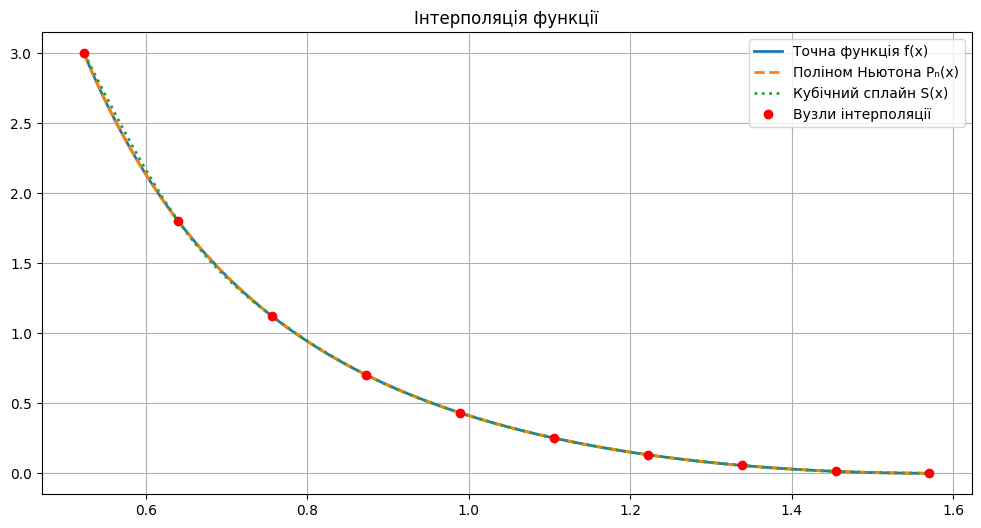
\includegraphics[scale=0.5]{Interpolation.png}
    \end{figure}

    \begin{figure}[h!]
        \centering
        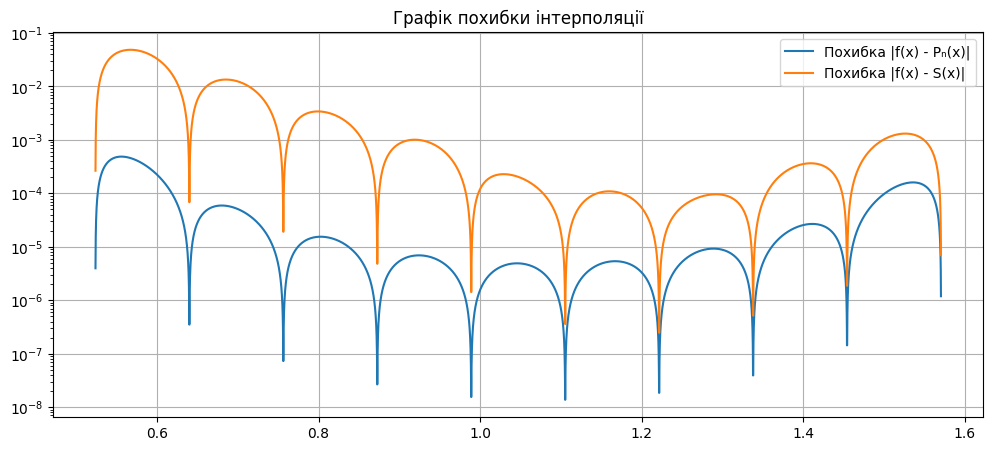
\includegraphics[scale=0.5]{Error.png}
    \end{figure}

\end{document}